\documentclass[%
%preprint,
 reprint,
superscriptaddress,
%groupedaddress,
%unsortedaddress,
%runinaddress,
%frontmatterverbose,
showpacs,preprintnumbers,
%nofootinbib,
%nobibnotes,
%bibnotes,
 amsmath,amssymb,
 aps,
 prl,
%pra,
%prb,
%rmp,
%prstab,
%prstper,
%floatfix,
]{revtex4-1}

\usepackage{siunitx}
\usepackage{graphicx}% Include figure files
\usepackage{dcolumn}% Align table columns on decimal point
\usepackage{bm}% bold math
\usepackage{hyperref}% add hypertext capabilities
\usepackage[mathlines]{lineno}% Enable numbering of text and display math
\usepackage{mathtools}
\linenumbers\relax % Commence numbering lines

%\usepackage[showframe,%Uncomment any one of the following lines to test
%%scale=0.7, marginratio={1:1, 2:3}, ignoreall,% default settings
%%text={7in,10in},centering,
%%margin=1.5in,
%%total={6.5in,8.75in}, top=1.2in, left=0.9in, includefoot,
%%height=10in,a5paper,hmargin={3cm,0.8in},
%]{geometry}
\DeclareSIUnit\basepair{bp}

\newcommand{\greens}[2][\Omega_0; L]{G(#2|#1)}
\newcommand{\pathd}[1]{\mathcal{D}\left[#1\right]}
\newcommand{\energy}{\mathcal{E}}
\newcommand{\wigD}{\mathcal{D}}
\newcommand{\RR}{\left\langle{}R^2\right\rangle{}}

\begin{document}
%\preprint{APS/123-QED}
\title{Heterogeneity in Nucleosome Spacing Governs Chromatin Elasticity}% Force line breaks with \\
\thanks{A footnote to the article title}%

\author{Bruno Beltran}
\thanks{These authors contributed equally to this work.}%
\affiliation{%
    Biophysics Program, Stanford University, Stanford, California 94305, USA
}%
\author{Deepti Kannan}%
\thanks{These authors contributed equally to this work.}%
\author{Quinn MacPherson}%
\affiliation{%
    Department of Physics, Stanford University, Stanford, California 94305, USA
}%
\author{Andrew J. Spakowitz}%
\email{ajspakow@stanford.edu}%
% \homepage{http://web.stanford.edu/~ajspakow/}%
\affiliation{%
    Chemical Engineering Department, Stanford University, Stanford, California 94305, USA
}%
% \altaffiliation[Also at ]{%
%     Department of Chemical Engineering, Stanford University, Stanford, California 94305, USA
% }%
\date{\today}% It is always \today, today,
             %  but any date may be explicitly specified

\begin{abstract}

%Start with a sentence leading into heterogeneity of proteins binding to DNA.
    In vivo, proteins that bind non-specifically to DNA introduce heterogenous
    kinks in the chromatin polymer.
    We propose a coarse-grained model for the effects of nucleosome packaging on the
    physical organization of chromosomal DNA, and present the analytical
    solution in the form of a Green's function.
Our analytical model combines a wormlike-chain treatment of the linker DNA
    connecting adjacent nucleosomes with the geometrical constraints imposed by
    DNA wrapping histone octamers.
The model predicts that adding realistic heterogeneity in the nucleosome spacing
    increases the elasticity of the chromatin chain relative to
    nucleosome-free DNA.% make this sentence evoke that the comparison is between individual chain
% instantiations
Furthermore, we find that rearranging nucleosome positions can cause the cell to
    change the looping probability of chromatin by up to 6 order of magnitude.
% if you're going to remove the first "increasing", you need to have some other
% way (you cna use more words) to evoke the idea that more variability makes the
% thing more like a random walk clearly
We demonstrate that these effects arise because increasing variability in
    nucleosome spacing forces the zero-temperature configuration of the fiber to
    increasingly resemble a random walk.
% "this geometric effect" now doesn't refer back to the word geometric as before
With just 1bp of variability in the nucleosome's binding positions,
    this geometrical effect overpowers thermal fluctuations in the WLC linkers.
Our framework fills a critical gap between models that explicitly incorporate
% i added back the word existing because, our model is also coarse grained.
% somethign should be done to make sure that this isnt' confusing, at least
    nucleosomes, but are computationally impractical to scale, and existing
    coarse-grained models of chromatin, which ignore the important contributions
    of nucleosome geometry.
In addition, our analytical approach is broadly applicable to any semiflexible
    polymer with aperiodic defects.
\end{abstract}

\pacs{05.20.--y, 05.40.Fb, 36.20.Ey, 87.10.Ca, 87.14.gk, 87.15--v, 87.16.Sr}% PACS, the Physics and Astronomy
                             % Classification Scheme.
%\keywords{Suggested keywords}%Use showkeys class option if keyword
                              %display desired
\maketitle

% examples of TOC and section headers left here for reference
%\tableofcontents
% \section{\label{sec:level1}First-level heading}
% \subsection{\label{sec:level2}Second-level heading: Formatting}

%HIGH LEVEL OUTLINE
%1. structure of genome matters (define nucleosome, brief intro on chromatin)
%2. heterogeneity plays a role in structure:
%in vivo DNA has high propensity for random binding that leads to random
%geometric organization;
%nucleosomes and other DNA-binding proteins (such as HU in bacteria) are not always perfectly spaced along the DNA
%3. Past analytical models of DNA have ommitted heterogeneity.
% two categories of analytical models: fixed NRL, or approximate chromatin as
% some effective wormlike chain to study local DNA mechanics (melting,
% kinking, helical WLC, etc.) DNA's mechanical properties will undeniably
% influence the various scales of physical behavior; however, approximating
% nucleosome-bound DNA as a homogenous polymer fails to account for the
% geometrical features that arise from heterogenous kinks imposed by
% nucleosomes or other DNA-binding proteins.
%4. In this paper, we present a model that includes the thermomechanical
%properties of DNA as well as aperiodic binding of nucleosomes. In the
%competition between these two factors, we find that the geometrical
%configuration of the fiber dominates thermal fluctuations in DNA linkers. We demonstrate
%that heterogeneity introduces order-of-magnitude differences in the elasticity
%of the polymer. We also find that these differences are not simply a composite
%average of the corresponding homogenous chains. We apply our model to the
%latest in vivo nucleosome positioning data to show that realistic variability
%in nucleosome spacing significantly affects the ability of chromatin to form
%loops, which is vital to transcriptional regulation

% \section{\label{sec:intro}Introduction}
In the cell, DNA and its associated proteins---collectively, chromatin---are
    carefully organized both spatially and temporally.
This organization is known to play a role in a myriad of biological processes,
    from gene expression to DNA damage repair, and has motivated a large body of work on the statistical mechanics of
    the chromatin fiber.

The fundamental repeating unit of Eukaryotic chromatin organization is the
    nucleosome, formed by 147 basepairs of DNA wrapped around a histone octamer.
Adjacent nucleosomes are connected by linker DNA, whose average length varies from
    $<$\SI{10}{\basepair} in some fission yeast [??] to over \SI{50}{\basepair} in
    many human cells [??].

While bare DNA is well described by a wormlike chain (WLC) with Kuhn length
    {$b = \SI{100}{\nano\metre}$}, few analytical models have attempted to
    incorporate nucleosomes into this picture.
% Increasingly realistic computational models of the chromatin fiber as a chain
%     of nucleosomes have been constructed in the past decade [Tamar-Schlick review].
% Unfortunately, these have always been limited to short chains with prespecified nucleosome
%     locations due to computational cost.
Past analytical efforts have only dealt with the special
    case of constant linker length, modeling chromatin as a WLC backbone and
    nucleosomes as periodic kinks [Koslover].
The constant linker length assumption was motivated by evidence
    that linker lengths are preferentially quantized [Widom92,Chereji18,others].
Moreover, models of helical chromatin fibers with fixed linker lengths
    [Grigoryev] reproduced the regularity of the well known ``\SI{30}{\nano\metre}
    fiber'' structure of \textit{in vitro} chromatin.

However, it is becoming increasingly clear that, \textit{in vivo}, nucleosome
    spacing is extremely heterogenous [nat chem meth paper on mnase, chereji, at
    least one eukaryotic alignment/phasing paper], even if some locations are
    statistically preferred.
Moreover, modern electron microscopy measurements suggest that \textit{in vivo} chromatin
    is largely disordered, contrary to the ``\SI{30}{\nano\metre} fiber''
    picture.
In an attempt to explain these measurements, recent simulation results have
    suggested that heterogeneity in nucleosome positioning might have unexpected
    effects on the structure of the fiber. [Tamar Schlick heterogeneity papers]
However, these detailed models are computationally expensive, and so they cannot
    provide broad guidance on how the fiber changes as a function of the nucleosome
    spacing distribution.
Due to this lack of theoretical guidance, it has become the \textit{de facto}
    standard to simply treat the chromatin fiber as if it were bare DNA for
    the purposes of coarse-grained simulations of the nucleus [Mirny, us,
    others].
%i'm not saying we should take this out, but i don't know what the point is
% you're tryign to make ehre, so maybe we should chat about it?
% Other  analytical models of DNA have focused on local deformations
    % of DNA due to kinking or melting.
% Although these contributions highlight the
    % importance of DNA's thermomechanical properties, they ignore the geometrical features that arise from heterogenous binding
    % of histones to DNA.

In this paper, we present an exact analytical treatment of a wormlike chain
    with arbitrarily spaced defects, and use it to investigate the effects of
    nucleosomes on chromatin structure.
We show that the elasticity of chromatin can be increased orders of magnitude by
    nucleosome binding, and that amount of this increase depends only on the average
    linker length for a given organism.
Furthermore, we show that aperiodic defects due to binding of nucleosomes---or, in
    practice, any protein that binds DNA---can change the
    propensity of two genomic loci encountering each other by up to six
    orders of magnitude.
Our results suggest that nucleosome positioning can affect not only
    accessibility and compaction, but also the mobility of a locus, and even
    the creation of functional chromatin loops.

%TODO, you had commented out only half of this sentence, did you just want to
    %delete it?
% Finally, we provide guidance for constructing coarse-grained models of chromatin
%     that account for the important effects of nucleosome heterogeneity
%     \textit{in vivo}.

More broadly, because none of our results depend on the particular properties of DNA or
    nucleosomes, we expect that our analytical approach will be broadly
    applicable a broad class of heterogenous polymers.
For example, block or random copolymers tend to be kinked at the junction
    between blocks, and we predict that this would cause a previously unexpected
    decrease in their Kuhn length.
% here's the closest thing I can say to Levy flights
Our work may also find application in models of driven gaussian processes,
    whenever driving events take place aperiodically.
%% I'd be stoked to mention conductive polymers, but not super clear on
%applications to random copolymers and conductive polymers, as well as models of complex
%% ah this is definitely not true, levy flights are just brownian motion with
%% heavy tailed step size distribution
%such as Levy flights

\section{\label{sec:model}Model}

We represent our polymer as a space curve $R(s)$, $s\in[0,L]$, along with a
    triad of vectors describing the chain's orientation at each location
    $\vec{t_i}$, where $\vec{t_3} \coloneqq R'(s)$.
We track the bend and twist of our polymer via the Euler vector $\omega_i$
    defined by $\partial_s \vec{t_i}(s) = \omega_i(s) \times \vec{t_i}(s)$.
The Green's function of the wormlike chain with twist starting at orientation
    $\Omega_0$, with length L, can then be written
\begin{equation}\label{eq:path}
    \greens{\vec{R}, \Omega} = \int_{s=0}^{s=L} \pathd{\Omega(s)}
              \delta\left(\vec{R} - \int_{s}^L \vec{t_3} ds\right)
              e^{-\beta \mathcal{E}},
    % overflows
    % \greens{\vec{R}, \Omega} = \int_{\Omega(s=0)}^{\Omega(s=L)} \pathd{\Omega(s)}
    %           \exp{[-\beta \mathcal{E}]}
    %           \delta\left(\vec{R} - \int_{s=0}^L \vec{t_3} ds\right)
\end{equation}
    where the energy
\begin{equation}\label{eq:energy}
    \beta\energy = \frac{l_p}{2}\int_{s=0}^L ds
    (\omega_1^2 + \omega_2 ^2) + \frac{l_t}{2}\int_{s=0}^L ds
    {\left(\omega_3 - \tau\right)}^2
\end{equation}
    is quadratic in bend and in twist, {$\tau \approx \SI{10.5}{\basepair}$}
    per turn is the equilibrium twist density of the DNA double helix, and {$l_p
    \approx \SI{50}{\nano\metre}$}, {$l_t \approx \SI{100}{\nano\metre}$} are
    the bend and twist persistence lengths of DNA, respectively.

This equation can be solved in Fourier space ($\vec{R} \rightarrow \vec{k}$) by
    expanding in Wigner D functions, the eigenfunctions of the heat equation on
    $SO(3)$~\cite{yamakawa1999}
% jump straight to B's, so we don't need the equation with g's here.
% \begin{equation}\label{eq:expansion}
%     \greens{\vec{k}, \Omega} = \sum_{l m j}\sum_{l_0 m_0 j_0} g_{l_0 m_0 j_0}^{lmj}
%         \wigD_l^{mj}(\Omega)\wigD_{l_0}^{m_0 j_0 *}(\Omega_0).
% \end{equation}
\begin{equation}\label{eq:expansion}
    \greens{\vec{k}, \Omega} = \sum_{l m j}\sum_{l_0 m_0 j_0} B_{l_0 m_0 j_0}^{lmj}
        \wigD_l^{mj}(\Omega)\wigD_{l_0}^{m_0 j_0 *}(\Omega_0).
\end{equation}
The coefficients $B_{l_0 m_0 j_0}^{lmj}(\Omega_\text{kink}, L)$ that define the
    propagator of a wormlike chain capped by a single, rigid kink were first
    computed
    % stole this citation from Lena's "systematic coarse graining" paper
    in~\cite{zhou2003}.
An alternate derivation can be found in the supplement.

\begin{figure}[t]
    \centering
    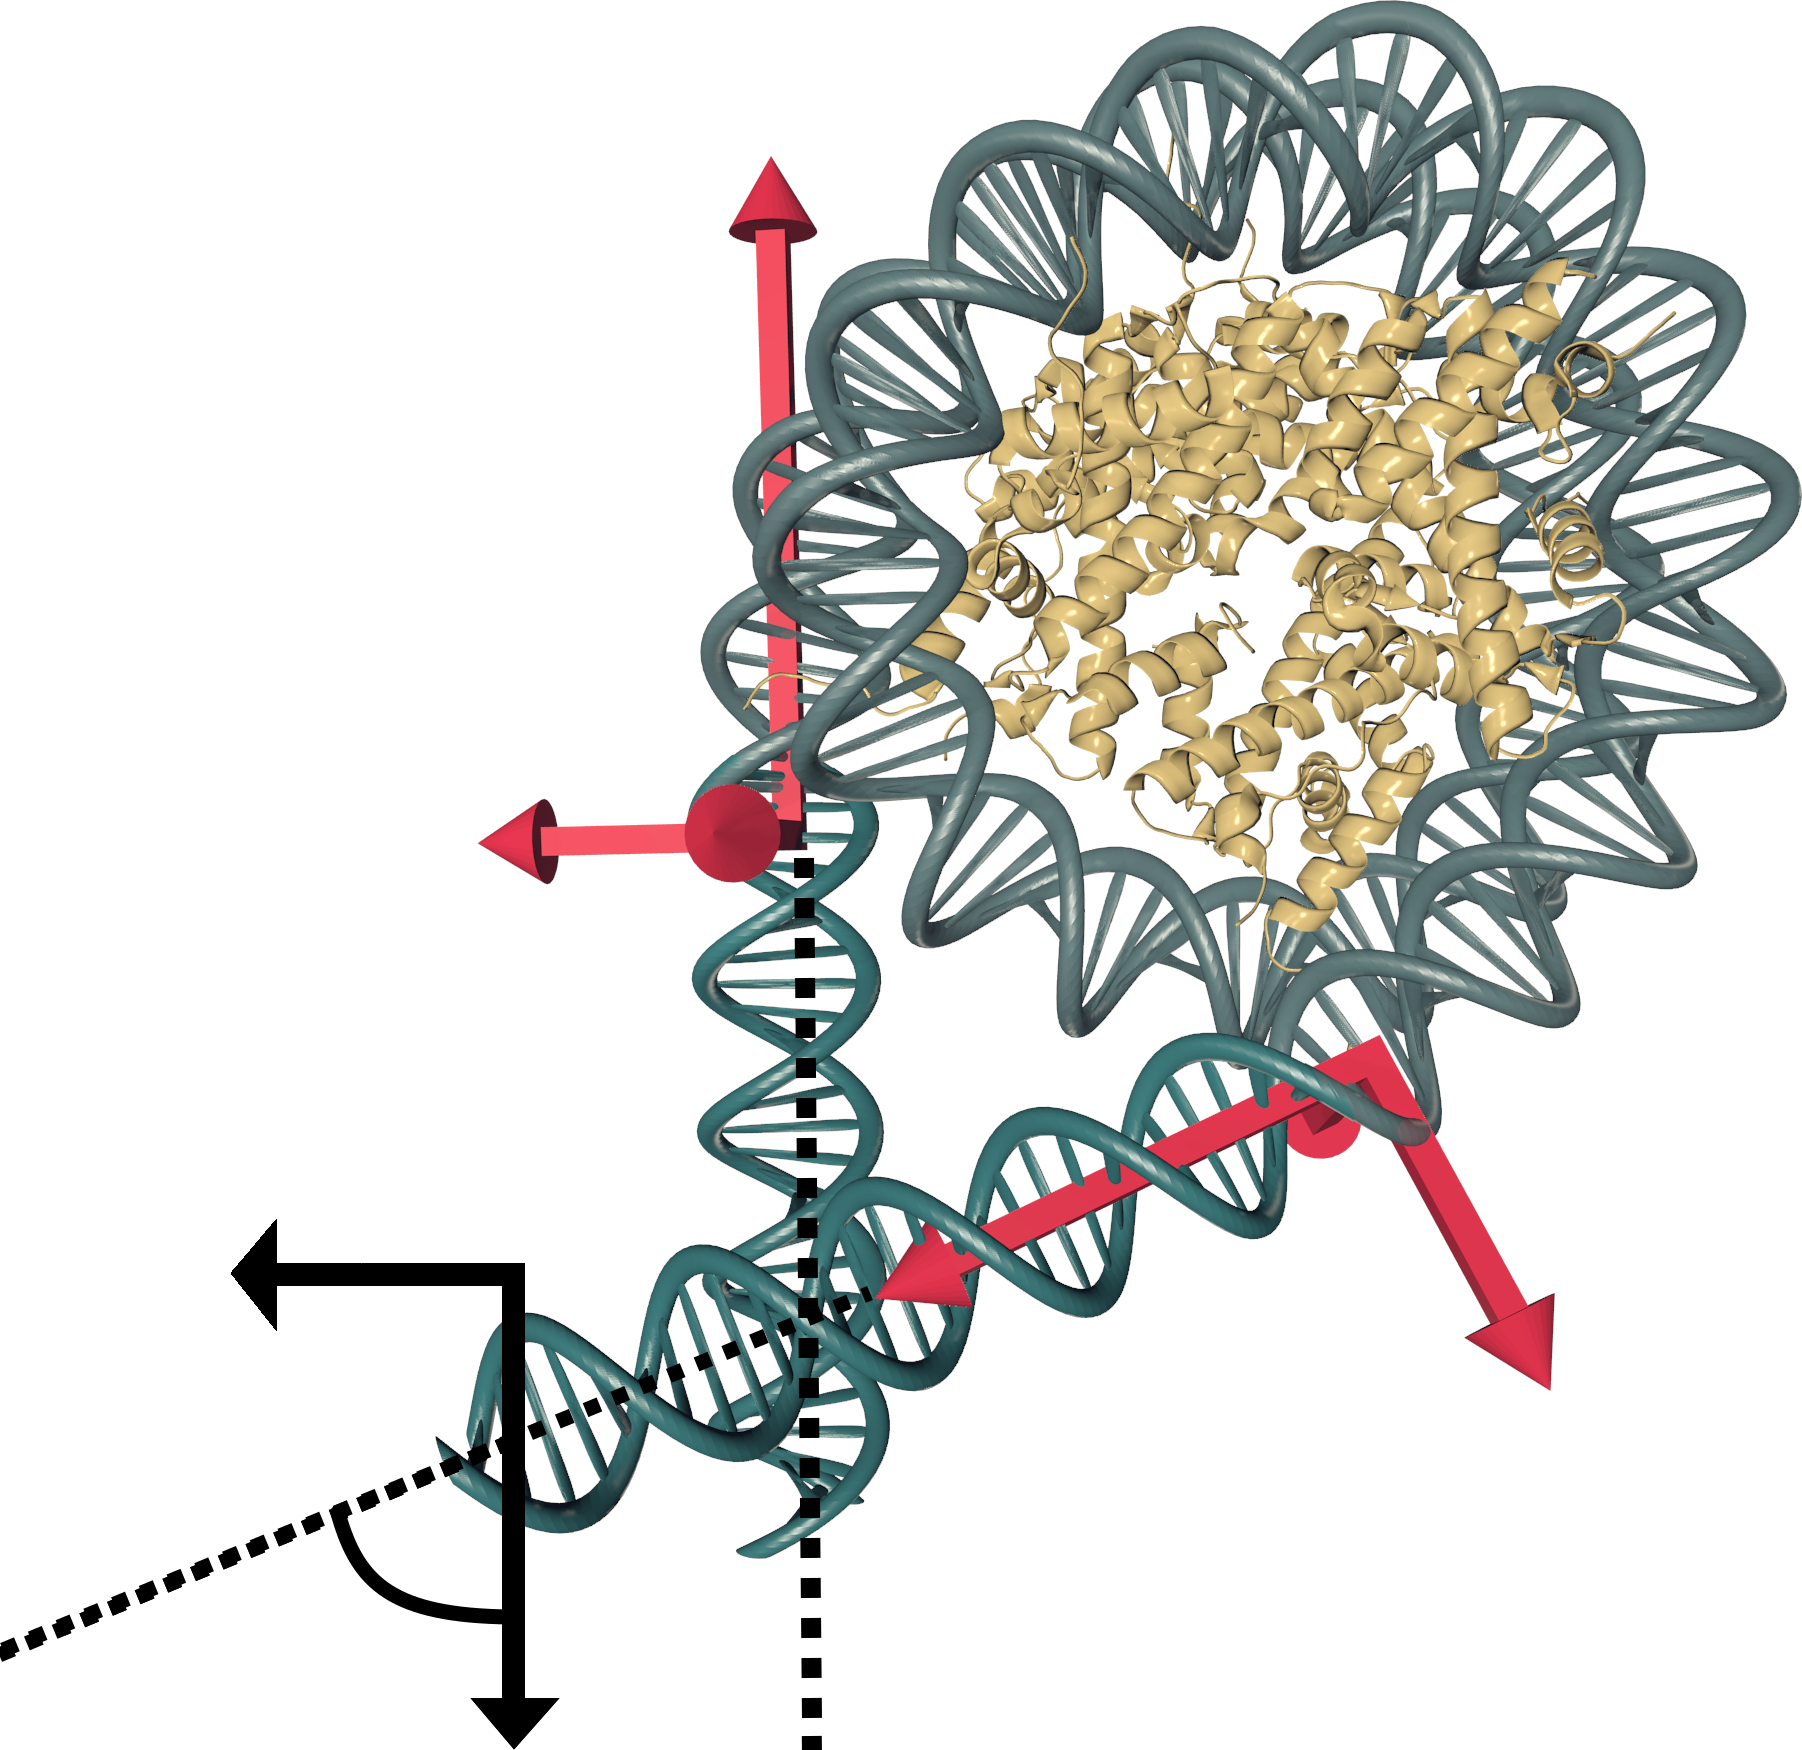
\includegraphics[width=0.35\linewidth]{./figures/fig-1a-nucleosome-geometry.png}
    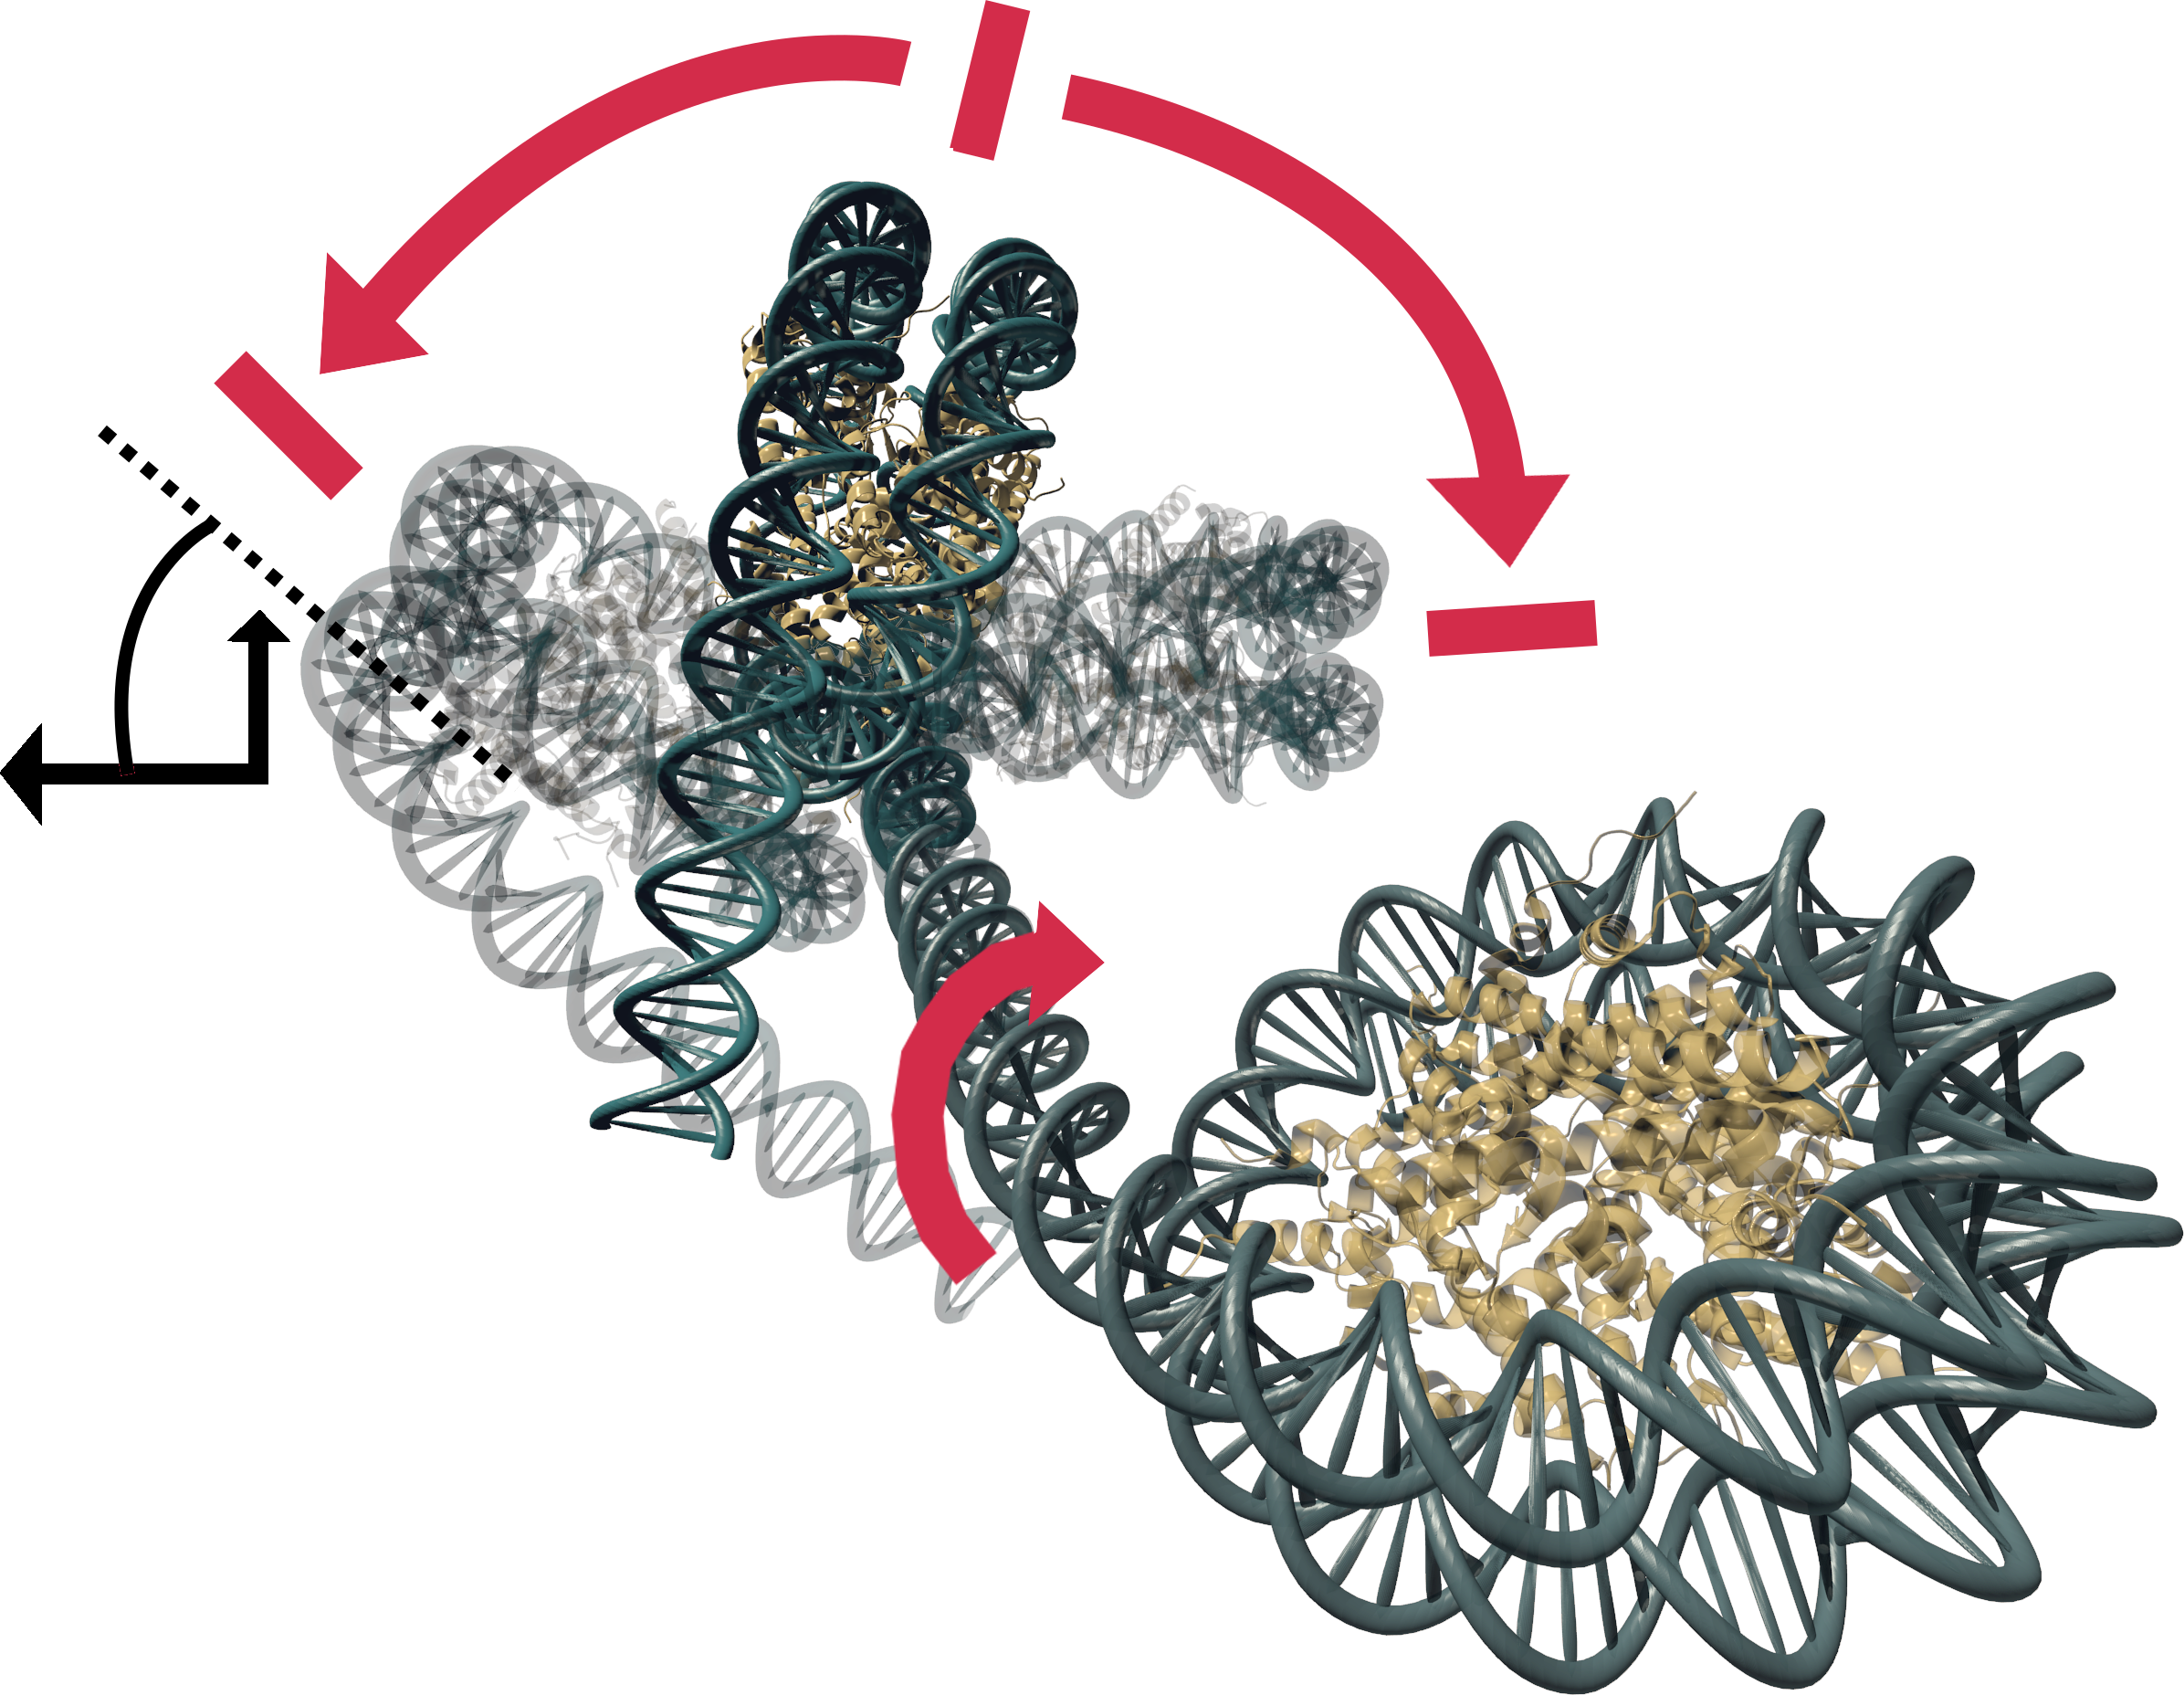
\includegraphics[width=0.52\linewidth]{./figures/fig-1b-helicity-effect.png}
    \caption{(a) When bound to a histone octamer, DNA traces out an
    approximately helical path. We treat the DNA bound to the histones as rigid,
    which corresponds to fixing the entry ($\Omega_\text{entry}$) and exit
    ($\Omega_\text{exit}$) orientations of the DNA from the nucleosome. Let
    ($\Omega_\text{nuc}(\theta, \phi)  =
    \Omega_\text{entry}^{-1}\Omega_\text{exit}$). The crystal structure of the
    nucleosome dictates the spherical angle $\theta$.
    (b) The DNA double helix has an intrinsic twist density
    $\tau=\SI{10.5}{basepair}$. At zero
    temperature, if we anchor the location of one nucleosome, the binding
    orientation of the next histone octamer must change so that it aligns with
    the major groove of the double helix. This means that as the linker length
    $l$ connecting two nucleosomes gets longer or shorter, the relative
    orientations of adjacent octamers changes by an angle $\phi = 2\phi l/\tau$.
    TODO:\@ include source of strcutre file (see bruno's file names).}\label{fig:nuc-geo}
\end{figure}

We extract the ``kink'' rotation $\Omega_\text{kink}$ describing the change in
    orientation of the DNA double helix due to binding the histone octamer from
    the nucleosome's structure (Figure~\ref{fig:nuc-geo}).
X-ray crystallography~\cite{white2001,richmond2003,cutter2015a} and
    %with H1: bednar, zhou; H4 acetlyation: wakamori; whole fiber: wakamori,
    %song2014b, eltsov2018, bilokapic.
    cryo-EM~\cite{bednar2017,bilokapic2018,eltsov2018,wakamori2015,zhou2015}
    measurements of the nucleosome have established that histone-bound DNA is
    well approximated by a deformed B-DNA structure, wrapping the histone
    octamer 1.7 times in a superhelix with radius \SI{4.19}{\nano\metre} and a
    pitch of \SI{2.59}{\nano\metre}~\cite{richmond2003}.

DNA is known to partially unwrap from the nucleosome core dynamically \textit{in
    vivo}, whether spontaneously (called nucleosome breathing~\cite{TODO}), due to
    force on the DNA~\cite{TODO}, or through active
    remodelling~\cite{dion2007,kulaeva2007,senavirathne2017}.
%While this process is important for allowing DNA-binding proteins to find
%DNA~\cite{polach1995,anderson2000,li2004}, transcript~\cite{kulaeva2007} and replication
%to take place...
In what follows, we fix the wrapping level to that found in the crystal
    structure.
% even though it has been directly measured through cryoem in solution that
    % nucleosomes are on average less wrapped than this~\cite{
Variability in nucleosome unwrapping can be easily incorporated into our model
    by drawing $\Omega_\text{nuc}$ from the appropriate distribution
We do not expect doing so would change the qualitative characteristics of our
    results.

In summary, the position and orientation of the $i$th nucleosome exit site
    is given by the convolution
\begin{equation}\label{eq:conv}
    \greens{\vec{R}, \Omega} = \greens[L_N]{\cdot} * \cdots{} *
    \greens[L_1](\cdot),
\end{equation}
where $L = \sum L_i$.
In Fourier space, this simply corresponds to multiplying the matrices $B^{(i)}$
    from Equation~\ref{eq:expansion}.

A key property of our model is that the relative orientation of adjacent
    nucleosomes is not just determined by $\Omega_\text{kink}$ and the thermal
    fluctuations of the linker strand.
%FINAL make sure the subfigure label matches final figure
As demonstrated in Figure~\ref{fig:nuc-geo}b, the length of the linker strand
    itself will change the relative orientation of two adjacent nucleosomes,
    even at zero temperature.
Our propagator $G$ takes this property into account implicitly thanks to the
    inclusion of $\tau$ in Eq.~\ref{eq:energy}.

Moments of the chain can simply be computed by noticing that
\begin{equation}\label{eq:moments}
    \lim_{k\to0} \frac{\partial^n B_{00}^{00}}{\partial k} = i^n \left\langle
    R^n\right\rangle
\end{equation}
See the Supplement for details.

Finally, to calculate the probability of two loci looping, we simply evaluate
    the aforementioned Green's function at $\vec{R} = 0$.
We note that this corresponds to a modified $J$ factor with no orientational
    component.

\begin{figure*}[th]
    \centering
    \includegraphics[width=0.15\textwidth]{./figures/fig-2b-mc-example.png}
    \includegraphics[width=0.325\textwidth]{./figures/fig-2a-kuhn-all.png}
    \includegraphics[width=0.5\textwidth]{./figures/fig-2c-kuhn-zoom.png}
    \caption{(a) The Kuhn lengths of homogenous chains are
    \SI{10.5}{\basepair} periodic
    in linker length, with each linker length representing a distinct,
    discretized helical
    WLC\@. In the limit of long linkers, the kuhn length eventually approaches that of bare DNA,
    \SI{100}{\nano\metre}. (b) Zero-temperature structure vs. Monte Carlo simulation
    snapshot of nucleosome chain with \SI{38}{\basepair} linkers. (c) Compact, superhelical structures afford more
    flexibility than non-compact fibres, which have higher Kuhn lengths. Thus,
    the overall structure of chromatin is extremely sensitive to changes in the
    nucleosome repeat length.}\label{fig:homo-kuhn}
\end{figure*}

\section{\label{sec:model}Results}
\subsection{\label{sec:homo-kuhn}Homogenous Nucleosome Spacing}

We begin by studying the illustrative, simple case of a homogenous chromatin
    chain, where there is a constant linker length separating adjacent
    nucleosomes.
Per Chasles's theorem, at zero temperature the nucleosomes in a homogenous chain
    form a superhelix (hereafter, the ``nucleosomal superhelix''\footnote{%
        This is distinct from the DNA superhelix that wraps each the nucleosome,
        which is in turn distinct from the intrinsic double helix of the
        underlying DNA itself.})
    whose compactness is determined by the angle between adjacent linkers, as
    shown in Figure~\ref{fig:homo-kuhn}a.
Because the angle between linkers depends on the linker length (again, see
    Figure~\ref{fig:nuc-geo}b), the shape of the nucleosomal helices formed by
    the homogenous chains depend on the linker length, as shown in
    Figure~\ref{fig:homo-kuhn}c.

We can use Eq.~\ref{eq:moments} to compute the mean squared displacement, $\RR$,
    of the homogenous chain as function of its linker length.
This allows us to extract the elasticity of homogenous chromatin via its Kuhn
    length, as shown in Figure~\ref{fig:homo-kuhn}b.
We note that due to Chasles's theorem, this calculation corresponds exactly to
    the kuhn length of the approriate discrete helical wormlike chain, as first
    done in~\cite{yamakawa1976}.

The discrete helical wormlike chain behaves similarly to a wormlike chain.
At short length scales, the $\RR$ behaves like a wormlike chain with reduced
    persistence length, due to the linkers being forced to traverse a helix.
At long length scales, the chain predictably asymptotes to a Gaussian
    chain, again with reduced Kuhn length compared to the underlying linkers.
It is noteworthy that the best fit persistence length at short scales and the
    best fit Kuhn length at long scales are quite different (Supplemental Figure
    XX).
Thus, our full theory is required even for calculations involving this
    simplified, homogenous chromatin chain.

We find that, to first approximation, the Kuhn length is determined by the
    amount of DNA contained per unit of rise along the nucleosomal superhelix,
    as shown in Figure~\ref{fig:homo-kuhn}c.
The bend and twist persistence lengths $l_p$ and $l_t$ of the linkers determine
    the average amount of bend and twist fluctuations in the linkers for each
    unit of distance along the DNA backbone.
Since the magnitude of the fluctuations is fixed in units of distance along the
    linkers, more compact structures, such as the \SI{36}{\basepair} and
    \SI{47}{\basepair} chains shown, will accumulate large fluctuations over a
    short distance along the nucleosomal superhelix.
On the other hand, in the more linear structures, such as \SI{41}{\basepair},
    the nucleosomal superhelix is approximately a straight line.
This means that for each unit of distance along the nucleosomal superhelix,
    there is less length of linker DNA, and, therefore, fluctuations accumulate
    more slowly, making the chain stiffer.

Perhaps most notably, the variability between the stiffest and most flexible
    chromatin chains spans over an order of magnitude in Kuhn lengths.
While some of the most compact configurations will sterically inaccesible, this
    already demonstrates the drastic effect that nucleosome binding can have on
    DNA's elasticity.

\subsection{\label{sec:homo-kuhn}Heterogenous Nucleosome $\RR$}

We now consider the more relevant scenario, when the nucleosomes are randomly
    spaced along the DNA backbone.
While certain DNA sequences have higher affinities for
    nucleosomes~\cite{something widom}, in practice the most striking features
    of nucleosome positioning data are nucleosome phasing near promoters, CTCF
    sites, and other sites that sterically inhibit nucleosome
    binding~\cite{widom1992}.
These features are predicted to occur by the simplest model of nucleosome
    positioning, one where nucleosomes are positioned uniformly along the DNA
    backbone, and simply sterically excluded from certain sites.
In terms of linker lengths, this model corresponds approximately to the case
    where linker lengths are independent and exponentially distributed about
    their mean.
Thus, while the exact statistics of \textit{in vivo} linker lengths remain to be
    determined, we use the case of I.I.D., exponentially distributed linkers as
    a reference point to show the effect of linker heterogeneity on the
    statistical mechanics of the chromatin fiber.





\begin{figure}[t]
    \centering
    \includegraphics[width=0.95\linewidth]{./figures/fig-3-box-variance.png}
    \caption{Kuhn lengths for zero-temperature configurations versus
    fluctuating linkers as a function of the amount of variance in the uniformly
    distributed linker lengths.  Adding \SI{6}{\basepair} of variability causes the zero-temperature
    configuration to resemble a random walk, explaining the reduced kuhn
    length predicted by the fullly fluctuating model. (b) For a mean linker
    length of \SI{47}{\basepair}, adding just \SI{1}{\basepair} of variance
    drastically reduces the kuhn length of the zero-temperature fiber.}
\end{figure}



\begin{figure}[t]
    \centering
    \includegraphics[width=0.95\linewidth,height=0.6\linewidth]{./figures/fig-4-exp-variance.png}
    \caption{Because sequence specificity of histone binding has a miniscule effect
    \textit{in vivo}, binding energies are approximately uniform across the
    genome. This leads to uniformly distributed nucleosome positions, with exponentially distributed linker lengths. We compare
    the kuhn lengths of realistic chromatin fibers against those of the
    corresponding zero-temperature configurations (red
    triangles) and bare
    DNA (dashed line). Geometrical kinks and fluctuations combine to drastically
    increase the elasticity of chromatin. Mean linker lengths in \textit{S.
    cerivisiae}[Chereji], mice embryonic stem cells [Voong], and human T cells
    [Valouev] are marked.}
\end{figure}


% THOUGHTS ON LOOPING
% Looping probabilities
% * Order of magnitude differences in variance at short length scales
% * Peak is at biological length scales (1 kB) —— moving nucleosomes around has a
% much bigger effect than elasticity of DNA
% * Everyone uses Rouse polymer at long length scales, but we’re showing that
% things aren’t Gaussian for a while…..
%     * Memory of kinks stays longer than in worm like chain
%     * Biophysics community has been trying to explain peaks in looping
%     probability at short chain lengths (J factor stuff) — can we explain this
%     with kinking and heterogeneity?
\begin{figure}[t]
    \centering
    \includegraphics[width=0.95\linewidth]{./figures/fig-5a-exp-looping.png}
    %\includegraphics[width=0.35\linewidth]{./figures/fig-5b-looping-features.png}
    \caption{(a) Each purple line designates an individual chain configuration
    with uniformly random linker lengths between 31 and \SI{51}{\basepair}, with
    the black line representing the average over individual chains. Thus, modulating nucleosome positions can allow the cell to change
    the probability of inter-nucleosomal contacts by up to 6 orders of
    magnitude. The peak in the average curve occurs at around a kilobase, the
    length scale of enhancer-promoter contacts. Although the average,
    heterogenous chain tends towards a Gaussian chain with a shorter
    effective Kuhn length, individual configurations retain memory of rigid kinks
    at intermediate length scales, as indicated by residual peaks in the looping
    probability.}
\end{figure}

\section{PRL Guidelines}

Must be submitted to a section, closest fit seems to be
L8--81: Biological and Medical Physics

Other options:
L0--06: Statistical Physics and Thermodynamics
L3--30: Dynamics and Structure of Atoms and Molecules
L6--60: Chemical Physics
but espeically these two:
L8--78: Liquid Crystals and Polymers


3750 words

Include:

Any text in the body of the article;
Any text in a figure caption or table caption;
Any text in a footnote or an endnote

Exclude:

Title;
Author and affiliation listing;
Abstract;
Receipt date, published date, and other publication history;
PACS or Keywords and DOI;\@
References;
Author byline footnotes;
Acknowledgments

Estimating the word equivalent for figures can be simplified by using the aspect
ratio (width / height) of the figure. The estimates would be ((150 / aspect
ratio) + 20 words) for single-column figures, and ((300 / (0.5 * aspect ratio))
+ 40 words) for double column figures.

The word equivalent for displayed math is 16 words per row for single-column
equations. Two-column equations count as 32 words per row.

% \section{\label{sec:level1}First-level heading}

% This sample document demonstrates proper use of REV\TeX~4.1 (and
% \LaTeXe) in mansucripts prepared for submission to APS
% journals. Further information can be found in the REV\TeX~4.1
% documentation included in the distribution or available at
% \url{http://authors.aps.org/revtex4/}.

% When commands are referred to in this example file, they are always
% shown with their required arguments, using normal \TeX{} format. In
% this format, \verb+#1+, \verb+#2+, etc. stand for required
% author-supplied arguments to commands. For example, in
% \verb+\section{#1}+ the \verb+#1+ stands for the title text of the
% author's section heading, and in \verb+\title{#1}+ the \verb+#1+
% stands for the title text of the paper.

% Line breaks in section headings at all levels can be introduced using
% \textbackslash\textbackslash. A blank input line tells \TeX\ that the
% paragraph has ended. Note that top-level section headings are
% automatically uppercased. If a specific letter or word should appear in
% lowercase instead, you must escape it using \verb+\lowercase{#1}+ as
% in the word ``via'' above.

% \subsection{\label{sec:level2}Second-level heading: Formatting}

% This file may be formatted in either the \texttt{preprint} or
% \texttt{reprint} style. \texttt{reprint} format mimics final journal output.
% Either format may be used for submission purposes. \texttt{letter} sized paper should
% be used when submitting to APS journals.

% \subsubsection{Wide text (A level-3 head)}
% The \texttt{widetext} environment will make the text the width of the
% full page, as on page~\pageref{eq:wideeq}. (Note the use the
% \verb+\pageref{#1}+ command to refer to the page number.)
% \paragraph{Note (Fourth-level head is run in)}
% The width-changing commands only take effect in two-column formatting.
% There is no effect if text is in a single column.

% \subsection{\label{sec:citeref}Citations and References}
% A citation in text uses the command \verb+\cite{#1}+ or
% \verb+\onlinecite{#1}+ and refers to an entry in the bibliography.
% An entry in the bibliography is a reference to another document.

% \subsubsection{Citations}
% Because REV\TeX\ uses the \verb+natbib+ package of Patrick Daly,
% the entire repertoire of commands in that package are available for your document;
% see the \verb+natbib+ documentation for further details. Please note that
% REV\TeX\ requires version 8.31a or later of \verb+natbib+.

% \paragraph{Syntax}
% The argument of \verb+\cite+ may be a single \emph{key},
% or may consist of a comma-separated list of keys.
% The citation \emph{key} may contain
% letters, numbers, the dash (-) character, or the period (.) character.
% New with natbib 8.3 is an extension to the syntax that allows for
% a star (*) form and two optional arguments on the citation key itself.
% The syntax of the \verb+\cite+ command is thus (informally stated)
% \begin{quotation}\flushleft\leftskip1em
% \verb+\cite+ \verb+{+ \emph{key} \verb+}+, or\\
% \verb+\cite+ \verb+{+ \emph{optarg+key} \verb+}+, or\\
% \verb+\cite+ \verb+{+ \emph{optarg+key} \verb+,+ \emph{optarg+key}\ldots \verb+}+,
% \end{quotation}\noindent
% where \emph{optarg+key} signifies
% \begin{quotation}\flushleft\leftskip1em
% \emph{key}, or\\
% \texttt{*}\emph{key}, or\\
% \texttt{[}\emph{pre}\texttt{]}\emph{key}, or\\
% \texttt{[}\emph{pre}\texttt{]}\texttt{[}\emph{post}\texttt{]}\emph{key}, or even\\
% \texttt{*}\texttt{[}\emph{pre}\texttt{]}\texttt{[}\emph{post}\texttt{]}\emph{key}.
% \end{quotation}\noindent
% where \emph{pre} and \emph{post} is whatever text you wish to place
% at the beginning and end, respectively, of the bibliographic reference
% (see Ref.~[\onlinecite{witten2001}] and the two under Ref.~[\onlinecite{feyn54}]).
% (Keep in mind that no automatic space or punctuation is applied.)
% It is highly recommended that you put the entire \emph{pre} or \emph{post} portion
% within its own set of braces, for example:
% \verb+\cite+ \verb+{+ \texttt{[} \verb+{+\emph{text}\verb+}+\texttt{]}\emph{key}\verb+}+.
% The extra set of braces will keep \LaTeX\ out of trouble if your \emph{text} contains the comma (,) character.

% The star (*) modifier to the \emph{key} signifies that the reference is to be
% merged with the previous reference into a single bibliographic entry,
% a common idiom in APS and AIP articles (see below, Ref.~[\onlinecite{epr}]).
% When references are merged in this way, they are separated by a semicolon instead of
% the period (full stop) that would otherwise appear.

% \paragraph{Eliding repeated information}
% When a reference is merged, some of its fields may be elided: for example,
% when the author matches that of the previous reference, it is omitted.
% If both author and journal match, both are omitted.
% If the journal matches, but the author does not, the journal is replaced by \emph{ibid.},
% as exemplified by Ref.~[\onlinecite{epr}].
% These rules embody common editorial practice in APS and AIP journals and will only
% be in effect if the markup features of the APS and AIP Bib\TeX\ styles is employed.

% \paragraph{The options of the cite command itself}
% Please note that optional arguments to the \emph{key} change the reference in the bibliography,
% not the citation in the body of the document.
% For the latter, use the optional arguments of the \verb+\cite+ command itself:
% \verb+\cite+ \texttt{*}\allowbreak
% \texttt{[}\emph{pre-cite}\texttt{]}\allowbreak
% \texttt{[}\emph{post-cite}\texttt{]}\allowbreak
% \verb+{+\emph{key-list}\verb+}+.

\bibliography{chromatin}

\end{document}
